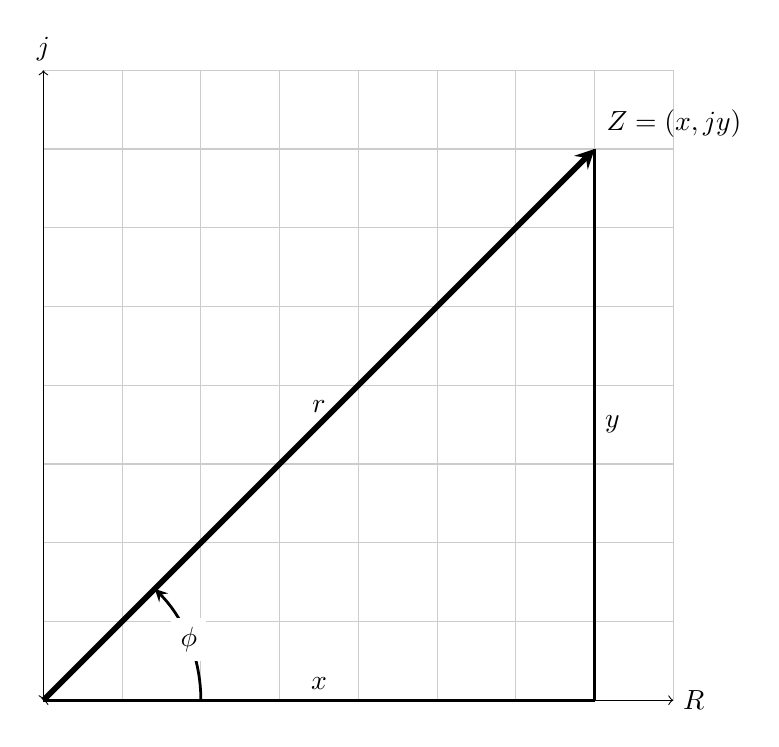
\begin{tikzpicture}
        \draw[thin,gray!40] (0,0) grid (8,8);
        \draw[<->] (0,0)--(8,0) node[right] {$R$};
        \draw[<->] (0,0)--(0,8) node[above]{$j$};
        \draw[line width=2pt,black,-stealth](0,0)--node[above]{$r$}(7,7) node[anchor=south west]{${Z=(x,jy)}$};
        \draw[line width=1pt,black,-](7,0)-- node[right]{$y$} (7,7);
        \draw[line width=1pt,black,-](0,0)-- node[above]{$x$}(7,0);
        \draw[line width=1pt,black,-stealth] (2,0) arc (0:45:2) node [midway,fill=white]{$\phi$};
\end{tikzpicture}
\caption{Planteo para la definición de la forma polar}